\chapter{Introduction}

The challenge of IPP is to find the optimal path that maximizes the information subject to budget constraints.
However, finding the optimal path is a NP-hard problem.
To solve these problems, some methods are proposed.
% Coverage-based planning is proposed to find a path that passes over all points of an area \cite{galceran2013survey}.
In \cite{popovic2017multiresolution}\cite{popovic2020informative}, the authors proposed an informative path planning framework in online settings with adaptivity requirements.
This approach enables agents to find a target based on the given constraints. However, these approaches cannot achieve the theoretical guarantees.



%{\color{olive}(Apply submodular function in IPP)}
Reformulating IPP problems as submodular maximization problems
is a promising approach with theoretical guarantees~\cite{nemhauser1978analysis}.
If the IPP problems can be reformulated as a maximizing submodular function subject to some constraints (e.g. cardinality~\cite{nemhauser1978analysis}, additive budget~\cite{khuller1999budgeted}, and routing~\cite{zhang2016submodular}), the variant greedy algorithms can give theoretical guarantees~\cite{nemhauser1978analysis}\cite{feige1998threshold}.

\begin{figure}[htbp]
\centering
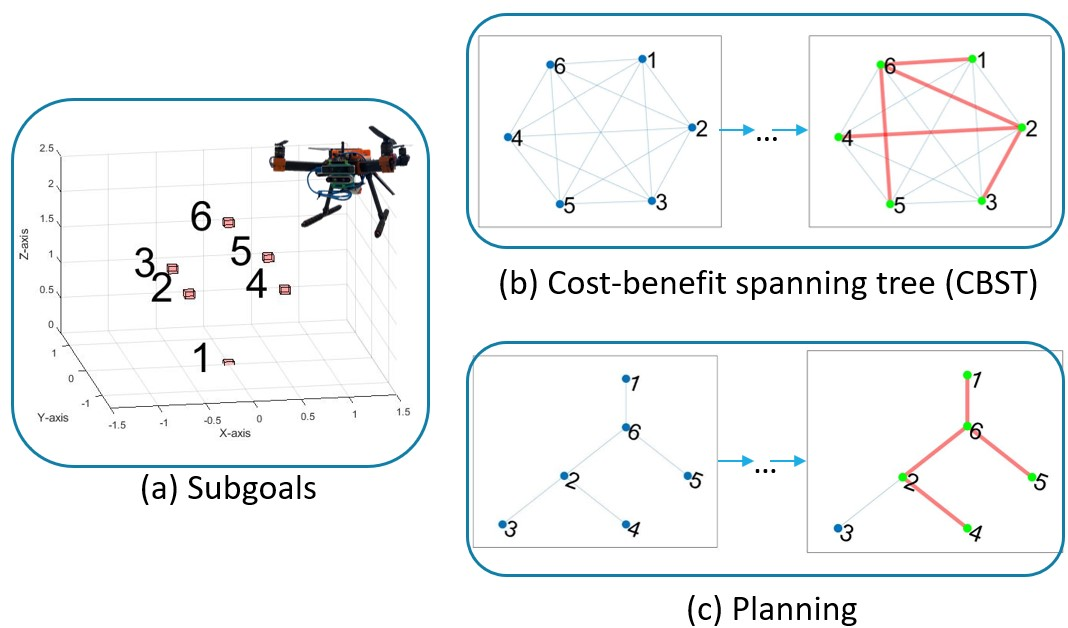
\includegraphics[width=1.0\linewidth]{method_intro.jpg}
\caption{ Illustration of the proposed method.
(a) Subgoals.
The blue points and decimal numbers represent subgoals and the index of subgoals, respectively.
(b) The cost-benefit spanning tree.
The green points, red lines and decimal numbers represent nodes in spanning tree, edges in spanning tree and the index of subgoals, respectively.
(c) Path.
The green points and red lines represent the path nodes and path edges, respectively.
}
%(b) The change of objective function from minimum spanning tree to cost-benefit spanning tree (c) Tree structure of \emph{CBST}.}
\label{fig:method_intro}
 \end{figure}

%{\color{olive}(GCB)}
The generalized cost-benefit (GCB) is proposed and proves the theoretical guarantees in the routing constraints~\cite{zhang2016submodular}, which is a traveling salesman problem (TSP) \cite{flood1956traveling}.
Hence, this problem includes two NP-hard problems.
First, that the agent finds the maximal information sets $K$ from $S$ sets~\cite{nemhauser1978analysis} is a set-covering problem~\cite{grossman1997computational}.
Second, that the agent finds the least route from $K$ subgoals is a TSP~\cite{lin1973effective}.
The GCB algorithm achieves $\frac{1}{2}(1-\frac{1}{e})\widetilde{OPT},$ where $\widetilde{OPT}$ is the approximation of optimum from the overestimated routing cost.
%{\color{olive}Since the TSP problem is NP-hard problem, it is infeasible to find the least cost route. The approximated solver for TSP is adopted, and it achieves a $\frac{3}{2}-$approximation ratio~\cite{christofides2022worst}. In~\cite{arora1996polynomial}, the researchers propose the algorithm, that is conjectured $\frac{4}{3}-$approximation, but it has been proven to be a worst-case upper bound~\cite{zambito2006traveling}.}

%{\color{olive}(The disadvantage of GCB and GCB-TSG)}
Since it is infeasible to find the least route from $K$ subgoals, the approximated algorithms are adopted for GCB. However, the approximated algorithms are overestimated.
It causes the GCB algorithm to terminate before utilizing all budgets.
%It achieves the $\frac{1}{2}(1-\frac{1}{e})\widetilde{OPT}$ guarantees, where $\widetilde{OPT}$ is the approximation of optimal solution.
%It is a gap between $\widetilde{OPT}$ and $OPT$.
The GCB-MST utilizes the submodularity of the spanning trees to boost the theoretical guarantee~\cite{lin2023improvement}.
The GCB and the GCB-MST achieve $\frac{1}{2}(1-\frac{1}{e})\widetilde{OPT}$ and $\frac{1}{2}(1-\frac{1}{e})\overline{OPT}$, respectively, where $\widetilde{OPT} \le \overline{OPT} \le OPT$, $\overline{OPT}$ is the approximation of optimum from submodular tree-structured graph cost.
%It achieves $\frac{1}{2}(1-\frac{1}{e})\overline{OPT}$, where $\widetilde{OPT} \le \overline{OPT} \le OPT.$
%If the tree structure is the shortest path tree (SPT) on the empty map, the theoretical guarantees achieve $\frac{1}{2}(1-\frac{1}{e})OPT.$

%{\color{olive} (The proposed approach with Fig.~\ref{fig:method_intro})}
The GCB-MST adopts the minimum spanning tree (MST) as the tree structure.
However, the MST could not be the best spanning tree.
To improve the performance, this research proposes cost-benefit spanning tree (CBST) algorithm, which generates subgoals as a cost-benefit objective.
As Fig.~\ref{fig:method_intro} (a) shows, there are $6$ nodes including $1$ source node (index $1$) in the map.
As Fig.~\ref{fig:method_intro} (b) shows, the approach using cost-benefit algorithm to span the tree.
As Fig.~\ref{fig:method_intro} (c) shows, the agent plans the path via greedy approaches.
% {\color{olive}In some cases, the important subgoals may be far from the starting point. It causes the agent to not be able to fly to important points if the budget is tight and the agent follows the MST.}
%{\color{red} (Try to make a better 1st figure. For example, there is a UAV. What's your approach? Illustrate it? )}

%Prim-Dijkstra (\emph{PD}) algorithm~\cite{alpert1993direct} can generate different types of spanning trees.
%As Fig.~\ref{fig:method_intro}(a) shows, there are six subgoals {\color{olive}on} this map.
%As Fig.~\ref{fig:method_intro}(b) shows, {\color{olive}the} Prim algorithm {\color{olive}on} this map generates the spanning tree.
%As Fig.~\ref{fig:method_intro}(c) shows, {\color{olive}the} Dijkstra algorithm {\color{olive}on} this map generates the spanning tree.
%In {\color{olive}the} \emph{PD} algorithm, {\color{olive}the parameters adjustment} causes different types of spanning. In Fig.~\ref{fig:method_intro}(b)(c), they are edge cases in {\color{olive}the} \emph{PD} algorithm.
%As Fig.~\ref{fig:method_intro}(d) shows, {\color{olive}the} \emph{PD} algorithm in this map generates various spanning trees.
%This research analyzes the performances of different types of spanning trees {\color{olive}on} the different maps.

%{\color{olive}(Contributions)}
The contributions of this research are as follows:
First, the informative path planning on terrain is reformulated as a submodular maximization problem with routing constraints.
The proposed algorithm, CBST, is able to solve this problem with theoretical guarantees.
Second, this research analyzes the performances of the different types of spanning trees.
Third, the experiments demonstrate that the proposed approaches outperforms the benchmark.

%{\color{olive}(Outline of this paper)}
The paper is organized as follows. Section 2 reviews the relevant work. Section 3 describes the background knowledge of this research. Section 4 introduces the problem formulation. Section 5 describes the proposed algorithms. Section 6 describes the experiments. Finally, Section 7 reports the conclusions and future work. 